\clearpage{\pagestyle{empty}\cleardoublepage}
%%%%%%%%%%%%%%%%%%%%%%%%%%%%%%%%%%%%%%%%%imposta l'intestazione di pagina
\lhead[\fancyplain{}{\bfseries\thepage}]{\fancyplain{}{\bfseries\rightmark}}
\pagenumbering{arabic}                  %mette i numeri arabi
\chapter{Stato dell'arte}
\section{Metadati}
I \textit{metadati} sono informazioni associate ad una pagina web o ad una porzione di essa che ne descrivono il contenuto, permettendo che i risultati delle ricerche degli utenti abbiano una maggiore efficacia.

Una volta definiti, i metadati possono essere condivisi e riutilizzati in più occasioni. Questo riutilizzo comporta i seguenti vantaggi:
\begin{itemize}
\item aumentare l'interoperabilità tra diversi sistemi che condividono dati e servizi.
\item ridurre i costi nello sviluppo di sistemi interoperabili, poiché il riutilizzo evita il trattamento delle ambiguità all'interno delle applicazioni.
\item facilitare il trattamento dei dati nei sistemi informativi in genere, ed in particolare in quelli che integrano e condividono dati, ad esempio, sistemi di supporto per il processo decisionale.
\end{itemize}

I metadati possono essere raggruppati o strutturati come “schemi di metadati”, un insieme di metadati progettati per uno scopo specifico, come la descrizione di un tipo di informazioni su una risorsa. La definizione o il significato degli elementi in sé è noto come semantica dello schema. I valori dati agli elementi dei metadati sono il suo contenuto. Gli schemi di metadati di solito specificano i nomi degli elementi e la loro semantica.

Per garantire un alto livello di consistenza dei contenuti, è possibile specificare regole di contenuto, ovvero linee guida che prescrivono quale tipo di informazione è registrata in ogni elemento di metadati, dove trovare le informazioni (es. da un'intestazione di pagina web, una didascalia di una fotografia, ecc.) e come l'informazione è formattata. 

Uno schema di metadati senza regole di sintassi stabilite è chiamato sintassi indipendente.

I metadati possono essere codificati in qualsiasi sintassi definibile come SGML, XML o JSON.

Gli schemi di metadati sviluppati e mantenuti da organizzazioni standard (come ISO) o organizzazioni che hanno assunto tale responsabilità (come la Dublin Core Metadata Initiative) sono chiamati standard di metadati.

I metadati sono generalmente classificati in tre tipi:
\begin{itemize}
\item \textit{metadati descrittivi}, descrivono una risorsa informativa per l'identificazione e il recupero attraverso elementi come titolo, autore e abstract.
\item \textit{metadati strutturali}, documentano le relazioni tra gli oggetti attraverso elementi come i collegamenti ad altri componenti (ad esempio, come le pagine vengono messe insieme per formare i capitoli).
\item \textit{metadati amministrativi}, aiutano a gestire le risorse informative attraverso elementi quali il numero di versione, la data di archiviazione e altre informazioni tecniche ai fini della gestione dei file, della gestione dei diritti e della conservazione.
\end{itemize}

\section{Metodi di generazione automatica di metadati}
Generare metadati di buona qualità in modo efficiente è essenziale per organizzare e rendere accessibile la grande quantità di risorse presente sul web. Il successo di biblioteche digitali, il sostenimento dell'interoperabilità e l'evoluzione del web semantico dipendono da una generazione di metadati efficiente\cite{metadata}.

\vspace{5mm}

L'utilizzo di strumenti automatici di generazione di metadati può facilitare la gestione di una quantità sempre crescente di informazioni.
Idealmente, questi strumenti sono capaci di estrarre informazioni da risorse strutturate e non strutturate, creando metadati di qualità che possano permettere interoperabilità semantica.

\vspace{5mm}

Tra i benefici delle generazione automatica di metadati vi è la scalabilità, per coprire la metadatazione di grandi quantità di informazioni che richiederebbe molto tempo se venisse gestita tutta manualmente, e la consistenza nella generazione dei dati.

A differenza della generazione manuale dei metadati, la generazione automatica dei metadati si basa su metodi automatici per assistere o completare il processo di creazione dei metadati. Greenberg ha distinto due metodi di generazione automatica dei metadati: l'estrazione dei metadati (\textit{metadata extraction}) e la raccolta dei metadati (\textit{metadata harvesting}).
L'estrazione dei metadati utilizza l'indicizzazione automatica e le tecniche di recupero delle informazioni per generare metadati strutturati utilizzando il contenuto originale delle risorse. La raccolta di metadati consiste invece nel raccogliere in modo automatico metadati già prodotti e archiviati da diversi repository.

\vspace{5mm}

All'interno di questa dicotomia di metodi di estrazione, vi sono molte tecniche più specifiche che i ricercatori hanno sviluppato per la generazione automatica di metadati. Polfreman et al. ha identificato sei tecniche che sono state sviluppate nel corso degli anni: \textit{raccolta di meta-tag}, \textit{estrazione di contenuti}, \textit{indicizzazione automatica}, \textit{text e data mining}, \textit{autogenerazione di dati estrinseci} e \textit{social tagging}. Sebbene l'ultima tecnica non sia propriamente una tecnica di generazione automatica di metadati, poiché viene utilizzata per generare metadati con un intervento minimo richiesto dai professionisti dei metadati, può essere vista come una possibile modalità per semplificare il processo di creazione dei metadati\cite{semi}.

\subsection{Estrazione di meta-tag}
L'\textbf{estrazione di meta-tag} è un processo dove vengono identificati valori per campi di metadati e popolati attraverso l'osservazione dei tag associati ai documenti, di fatto convertendo i metadati raccolti da più repository in formati diversi.

La più grande debolezza di questo tipo di tool è il fatto che la sua efficacia dipenda dalla qualità dei metadati raccolti.
Tra i tool che sfruttano questa tecnica vi sono MarcEdit, che mediante appositi harvester raccoglie metadati da record conformi al protocollo \textbf{Open Archives Initiative Protocol for Metadata Harvesting} (\textbf{OAI-PMH}) e che può convertire in diversi formati (MARC, MARC XML, MODS, EAD), e tool come Editor-Converter Dublin Core Metadata e Firefox Dublin Core Viewer Extension che convertono informazioni trovate nei meta-tags dei file HTML trovati sul web in elementi Dublin Core.

L'OAI-PMH fornisce un framework di interoperabilità, indipendente dall'applicazione, basata sul raccoglimento dei metadati. Il framework di OAI-PMH comprende i service provider, che eseguono richieste per effettuare la raccolta dei metadati, e i data provider, che espongono i metadati. OAI-PMH è largamente utilizzato da biblioteche digitali, repository istituzionali e archivi digitali\cite{harvesting}. Alcuni esempi di archivi che implementano OAI-PMH sono:

\begin{itemize}
\item Digital Public Library of America (DPLA), aggrega metadati relativi a enti istituzionali americani
\item National Science Digital Library (NSDL), è un libreria digitale ad accesso libero contenente collezioni di metadati inerenti a scienze, tecnologia, ingegneria e matematica
\item OAIster, un catalogo di milioni di record relativi a risorse di fonti eterogenee
\item Open Language Archives Community (OLAC), una libreria virtuale di risorse linguistiche
\end{itemize}

\subsection{Estrazione di contenuti}
L'\textbf{estrazione di contenuti} è una forma di estrazione di metadati che sfrutta algoritmi di machine learning per associare parole chiave al documento sulla base del suo contenuto. Il vantaggio di questo approccio è che il risultato è indipendente dalla qualità dei metadati associati alla risorsa. Esempi di applicazioni che impiegano questa tecnica sono Kea, che utilizza le tecniche TF-IDF e first-occurence per identificare e assegnare frasi chiave da risorse testuali, e Open Text Summarizer che esegue l'estrazione automatica di un riassunto del testo passato in input e delle relative parole chiave. 

I metodi di estrazione di parole chiave possono essere suddivisi in tre categorie: metodi statistici, metodi basati sui grafi e metodi basati sul deep learning\cite{extraction}.

\subsection{Metodi statistici}
I \textbf{metodi statistici} sono i più semplici. Calcolano le statistiche per le parole chiave e utilizzano tali statistiche per valutarle. Tra questi metodi rientrano il calcolo la frequenza delle parole, la collocazione linguistica, la co-occorrenza e tecniche più sofisticate come TF-IDF e YAKE!.

\textbf{TF-IDF} (Term Frequency–Inverse Document Frequency) stima l'importanza della parola nel documento rispetto all'intero corpus (insieme di più documenti). Calcola la frequenza di ogni termine nel documento e la pondera con l'inverso della frequenza del termine nell'intero corpus. Le parole chiave verranno selezionate tra i termini con i punteggi più alti. Questo algoritmo favorisce i termini frequenti nel documento di testo e non frequenti negli altri documenti. Il vantaggio di TF-IDF è che è veloce e lo svantaggio è che necessita di un corpus di almeno qualche dozzina di documenti. TF-IDF è indipendente dalla lingua.

\textbf{YAKE!} (Yet Another Keyword Extractor) è un metodo di estrazione di parole chiave che utilizza feature statistiche ricavate da un singolo documento per estrarre le parole chiave. Estrae le parole chiave in cinque passaggi:
\begin{enumerate}
\item \textbf{Pre-elaborazione e identificazione del termine candidato}: il testo è suddiviso in frasi, blocchi (parte della frase separata da punteggiatura) e token. Il testo viene pulito, etichettato e vengono identificate le stop words.
\item \textbf{Estrazione delle caratteristiche}: calcola le seguenti cinque feature statistiche per i termini (parole) nel documento:
\begin{itemize}
\item Casing: conta il numero di volte (in proporzionale al numero complessivo di volte in cui compare) in cui il termine appare in maiuscolo o come acronimo nel testo. Un termine significativo di solito appare più spesso in maiuscolo.
\item Posizione del termine: posizione mediana della frase del termine nel testo. I termini più vicini all'inizio tendono a essere i più significativi.
\item Normalizzazione della frequenza dei termini: misura la frequenza bilanciata dei termini nel documento.
\item Relazione del termine al contesto: misura con quanti termini diversi il termine candidato coesiste. Termini più significativi coesistono con meno termini diversi. 
\item Termine in frasi diverse: misura quante volte i termini compaiono in frasi diverse. Un punteggio più alto indica un termine più significativo.
\end{itemize}
\item \textbf{Calcolo del punteggio del termine}: le funzioni del passaggio precedente vengono combinate in un unico punteggio.
\item \textbf{Generazione di n-grammi e calcolo dei punteggi delle parole chiave}: l'algoritmo identifica tutti gli n-grammi validi. Le parole negli n-grammi devono appartenere allo stesso blocco e non devono iniziare o terminare con una stopword. Successivamente, ogni n-gramma viene valutato moltiplicando i punteggi dei suoi membri e normalizzato per ridurre l'impatto della lunghezza dell'n-gramma. Le stopword vengono trattate in modo diverso per ridurre al minimo il loro impatto.
\item \textbf{Deduplicazione e ranking dei dati}: vengono rimosse le parole chiavi simili tra loro.
\end{enumerate}

\subsection{Metodi basati sui grafi}
I metodi basati su grafi generano un grafo dei termini correlati presenti nei documenti. Un grafo, ad esempio, può collegare i termini che si verificano contemporaneamente nel testo. I metodi basati su grafi utilizzano metodi di classificazione che considerano la struttura del grafo per valutare l'importanza del vertice. Uno dei metodi di questa categoria più conosciuti è TextRank.

\textbf{TextRank} è un metodo di classificazione basato su grafi utilizzato per estrarre frasi pertinenti o trovare parole chiave. L'estrazione delle parole chiave avviene in cinque passaggi:

\begin{itemize}
\item \textbf{Tokenizzazione e annotazione del testo} con tag di Part of Speech (PoS) (nomi, articoli, verbi...)
\item \textbf{Costruzione del grafo di co-occorrenza di parole}: i vertici nel grafo sono parole con tag PoS selezionati. Due vertici sono collegati con un arco se compaiono all'interno della finestra di N parole nel testo. Il grafo è non orientato e non ponderato.
\item \textbf{Graph ranking}: partendo con il punteggio di ciascun vertice inizializzato a 1, viene applicato sul grafo l'algoritmo di ranking utilizzando la seguente equazione:
\begin{equation}
S(Vi)=(1 - d) + d\left (\sum_{j \in In(Vi)} \frac{S(Vj)}{|Out(Vj)|}\right )
\end{equation}
Il peso \textit{S(Vi)} di un vertice \textit{Vi} è calcolato considerando i pesi dei vertici connessi al nodo \textit{Vi}. Nell'equazione, \textit{d} è il fattore di smorzamento impostato su 0,85. Gli \textit{In(Vi)} corrispondono ai collegamenti in entrata al vertice \textit{Vi} e gli \textit{Out(Vj)} ai collegamenti in uscita dal vertice \textit{Vj}. Poiché stiamo considerando grafi non orientati, un collegamento in entrata verso un nodo è anche un collegamento in uscita dallo stesso nodo. L'algoritmo viene eseguito su ciascun nodo in diverse iterazioni fino a quando i pesi sui nodi convergono: la variazione tra le iterazioni è inferiore a 0,0001.
\item \textbf{Selezione delle parole con il punteggio più alto}: le parole (quindi i vertici) sono ordinate per punteggio, dal più alto al più basso. Viene poi selezionato il primo terzo delle parole.
\item \textbf{Estrazione delle parole chiave}: in questo passaggio, le parole selezionate nella fase precedente vengono unite in parole chiave composte da più parole se compaiono in una stessa frase. Il punteggio delle parole composte corrisponde alla somma dei punteggi delle parole singole che le compongono.
\end{itemize}

L'algoritmo viene eseguito su ciascun documento separatamente e non necessita di un corpus di documenti per eseguire l'estrazione delle parole chiave. TextRank è indipendente dalla lingua.

\textbf{RAKE} (Rapid Automatic Keyword Extraction) è un altro algoritmo di estrazione delle parole chiave basato su grafi. L'algoritmo si basa sull'osservazione che le parole chiave sono spesso composte da più parole e di solito non includono stop-word o punteggiatura.

Include i seguenti passaggi:
\begin{itemize}
\item \textbf{Estrazione delle parole chiave candidate}: il testo viene suddiviso in base alle parole chiave candidate in base alle parole di arresto e al delimitatore di frase. Una parola chiave candidata è una frase che si trova tra due stop-word o delimitatori di frase. I delimitatori di frase sono, ad esempio, i caratteri di punteggiatura.
\item \textbf{Costruzione del grafo di co-occorrenza delle parole chiave}: i vertici nel grafo corrispondono a parole. Sono collegati se compaiono insieme nelle parole chiave candidate. Il grafo è ponderato: il peso corrisponde al numero di volte in cui le parole collegate appaiono insieme nelle parole chiave candidate. Un vertice può essere collegato a sé stesso nel caso corrisponda a una parola che appare in una parola chiave candidata insieme a sé stessa.
\item \textbf{Punteggio delle parole}: ogni parola nel grafo è valutata con uno dei seguenti punteggi: 
\begin{itemize}
\item \textit{Grado della parola} (\texttt{deg(w)}): numero di parole con cui la parola w co-occorre (somma dei pesi degli archi). Il grado favorisce le parole che compaiono più spesso e in parole chiave più lunghe.
\item \textit{Frequenza della parola} (\texttt{freq(w)}): numero di volte che la parola appare in qualsiasi parola chiave candidata. Questo criterio favorisce le parole che appaiono più frequentemente.
\item \textit{Rapporto tra grado e frequenza} (\texttt{deg(w)/freq(w)}): favorisce le parole che ricorrono principalmente nelle parole chiave candidate più lunghe. Il grado favorirà le parole chiave più brevi.
\end{itemize}
\item \textbf{Punteggio delle parole chiave candidate}: il punteggio di ciascuna parola chiave candidata è la somma dei punteggi delle parole che la compongono.
\item \textbf{Parole chiave adiacenti}: le parole chiave candidate non includono stopword. Poiché a volte le stopword possono essere parte della parola chiave, vengono aggiunte in questo passaggio. L'algoritmo individua le coppie di parole chiave di cui fa parte almeno una stopword e, nel caso quest'ultima sia presente almeno due volte nel testo, le aggiunge all'insieme delle stopword esistenti. Il punteggio della nuova parola chiave è la somma dei punteggi delle parole chiave che la compongono.
\item \textbf{Estrazione delle parole chiave}: viene infine estratto il terzo delle parole chiave con il punteggio migliore.
\end{itemize}

La differenza principale tra RAKE e TextRank è che RAKE considera le ricorrenze all'interno delle parole chiave candidate invece di una finestra fissa. Utilizza una procedura di punteggio più semplice e statistica: non include l'ottimizzazione. L'algoritmo viene eseguito su ciascun documento separatamente, quindi non necessita di un corpus di documenti.

\subsection{Metodi basati sul deep learning}
La comparsa del deep learning ha consentito metodi basati sull'embedding, un insieme di tecniche di modellazione in cui le parole vengono mappate in vettori di numeri reali. 

Questi metodi trovano principalmente un elenco di parole chiave candidate (ad esempio, Bennani et al. considerano solo parole chiave costituite da nomi e aggettivi). Incorporano il documento e le parole chiave candidate nello stesso spazio di inclusione e misurano la similarità (ad es. similarità del coseno) tra i valori del documento e delle parole chiave. Selezionano le parole chiave più simili al testo del documento in base alla misura di similarità.

\subsection{Indicizzazione automatica}
Così come la content extraction, l'\textbf{indicizzazione automatica} prevede l'utilizzo di machine learning e algoritmi rule-based per estrarre metadati dalle risorse. La differenza sta nel fatto che i termini estratti vengono successivamente mappati in vocabolari controllati come Library of Congress Subject Headings (LCSH), Getty Thesaurus of Geographic Names (TGN), Library of Congress Name Authority (LCNA) o ontologie relative a un dominio specifico. I termini determineranno possibili punti di accesso sotto i quali i documenti associati possono essere cercati e identificati.

Il processo di indicizzazione si compone di tre fasi:
\begin{itemize}
\item analisi del documento e individuazione del suo tema di base (il contenuto concettuale).
\item identificazione dei concetti principali presenti in tale contenuto (l'insieme di tali concetti costituisce il "soggetto" del documento stesso).
\item traduzione nei termini di un linguaggio di indicizzazione, utilizzando termini estratti dal documento stesso (indicizzazione derivata, o estratta) oppure avvalendosi di un dizionario controllato ("indicizzazione assegnata")
\end{itemize}

\subsection{Text e data mining}
A causa della complessità delle tecniche utilizzate per l'estrazione di metadati, la maggior parte degli usi di queste tecniche sono stati sviluppati per risolvere i problemi della generazione automatica di metadati nel contesto di specifici progetti di ricerca.
I principali motivi sono il fatto che l'efficacia di queste tecniche dipende dalla qualità e dalla quantità dei dati di training, e che i vocabolari controllati come LCSH sono troppo complicati e diversificati per essere applicati con mezzi automatici.

\subsection{Autogenerazione di dati estrinseci}
La generazione automatica di dati estrinseci è il processo di estrazione dei metadati su una risorsa informativa che non è contenuta all'interno della risorsa stessa. La generazione automatica di dati estrinseci può includere l'estrazione di metadati tecnici come il formato e le dimensioni del file, ma può essere anche l'estrazione di funzionalità più complesse come il livello di classe scolastica a cui è destinata una risorsa educativa o il tipo di lettori per cui è destinato un documento.
Processi di questo tipo sono difficili da implementare a causa dell'assenza di informazioni sul contesto di una risorsa
contenute nella risorsa stessa.
Tra i tool che implementano questa tecnica di estrazione di metadati vi sono Dspace e JHove.

\subsection{Social Tagging}
Il social tagging è una forma di generazione di metadati, sebbene non propriamente automatica, che permette agli utenti di creare e assegnare tag alle risorse di un sito web. A causa del costo relativamente basso della generazione e del mantenimento dei metadati attraverso il social tagging e della sua attuale popolarità diffusa, alcuni progetti hanno tentato di utilizzare questi dati per migliorare i repository di archiviazione di metadati. Ad esempio, Linstaedt et al. usa sofisticati programmi per computer per analizzare le immagini statiche trovate all'interno di Flickr e utilizzare questi risultati d'analisi per propagare tag utente pertinenti a nuove immagini elaborate.

Un esempio di utilizzo del social tagging più complesso può consistere nell'utilizzare tecniche di apprendimento automatico, tenendo traccia dei cambiamenti applicati sui metadati associati a una risorsa da parte degli utenti e migliorare quindi i meccanismi di learning del database sulla base di queste modifiche.
Tra i tool che supportano il social tagging vi sono Dspace e Omeka.

Sebbene gli strumenti di generazione automatica di metadati offrano molti vantaggi, soprattutto per quanto riguarda la semplificazione del processo di creazione dei metadati, esistono barriere significative all'adozione e all'implementazione diffusa di questi strumenti. Un problema incontrato con gli strumenti di generazione automatica di metadati è che molti di essi sono sviluppati localmente per soddisfare le esigenze specifiche di un determinato progetto o come parte della ricerca accademica.

Diversi tool sono focalizzati alla risoluzione di pochi problemi specifici legati alla generazione di metadati, come possono essere l'estrazione di parole chiave di Kea piuttosto che l'estrazione di tag HTML e la successiva conversione in elementi Dublin Core di Editor Converter Dublin Core, portando quindi a sforzi significativi per coordinare le applicazioni selezionate e ottenere l'output desiderato.
È inoltre necessaria una buona conoscenza tecnica di linguaggi di programmazione per implementare questi sistemi propriamente.

Un altro problema è la discontinuità delle applicazioni, che possono presto risultare obsolete e perdere supporto tecnico.

\section{Ricerca sul tema}
Gli sforzi di ricerca per la generazione automatica di metadati possono essere classificati in due aree: \textbf{ricerca sperimentale}, focalizzata sulle tecniche di recupero delle informazioni e sui contenuti delle risorse digitali, e \textbf{ricerca applicativa}, riguardante lo sviluppo di software per la creazione di contenuti e strumenti di generazione di metadati utilizzati nel contesto operativo\cite{amega}.

\subsection{Ricerca sperimentale}
La crescita dei repository di risorse digitali fornisce una grande quantità di collezioni per lo studio della generazione automatica di metadati.

I ricercatori che gestiscono il contenuto delle risorse digitali per la generazione di metadati hanno sperimentato principalmente con la \textbf{struttura dei documenti} e i \textbf{sistemi di rappresentazione della conoscenza}.

\subsubsection{Struttura del documento}
I ricercatori hanno identificato relazioni tra genere, contenuto e struttura del documento. Ad esempio, il genere del documento può dare informazioni sulla densità testuale, che può essere utilizzata per prevedere le prestazioni dell'algoritmo di estrazione dei metadati per determinati tipi di documenti.

Il genere del documento inoltre determina una struttura prevedibile che facilita l'estrazione automatica di metadati. Ad esempio, i documenti di ricerca includono informazioni standard come "titolo", "autore" e "affiliazione dell'autore del documento. Gli esperimenti che sfruttano la struttura del documento in questa seconda sede utilizzando un algoritmo Support Vector Machine (SVM) (ad esempio, Han et al., 2003) e Variable Hidden Markov Model (DVHMM) (Takasu, 2003) hanno avuto un discreto successo per la generazione di metadati.

\subsubsection{Sistemi di rappresentazione della conoscenza}
La memorizzazione di metadati può essere eseguita attraverso l'utilizzo di ontologie, thesauri, sistemi classificatori, file di autorità e altri strumenti di rappresentazione della conoscenza.
Attraverso l'utilizzo di regole di inferenza, è possibile generare ulteriori informazioni relative a un oggetto sulla base dei valori delle sue proprietà.

\subsection{Ricerca applicativa}
Tra gli strumenti in grado di generare automaticamente metadati è possibile distinguere i software per la creazione di contenuti da tool più specializzati conosciuti come applicazioni per la generazione di metadati.

\subsubsection{Software per la creazione di contenuti}
Esempi di software per la creazione di contenuti sono Microsoft Word, Adobe Acrobat e Nullsoft Winamp, essenzialmente qualsiasi software che può essere utilizzato per creare contenuti digitali, testuali o multimediali. Nel contesto del web, il software per la creazione di contenuti viene utilizzato per creare una risorsa digitale a cui è possibile accedere tramite un browser e il software associato. Anche un surrogato bibliografico può essere considerato contenuto.

I software per la creazione di contenuti possono supportare la generazione di metadati tramite mezzi automatici, semiautomatici e umani. Le tecniche automatiche sono spesso impiegate per produrre metadati tecnici come la data di creazione, la data dell'ultima modifica, la dimensione in byte e il formato del file.

Alcuni software per la creazione di contenuti estraggono i metadati dal contenuto del documento nel tentativo di fornire rappresentazioni descrittive (ad esempio, Word assegna automaticamente un titolo in base alla prima riga di un documento). Alcuni software per la creazione di contenuti includono un modello per facilitare l'immissione di metadati umani. Le tecniche automatiche possono quindi essere impiegate dall'applicazione per convertire i metadati immessi in un linguaggio di codifica specificato, incorporarli in un'intestazione di risorsa o inserirli in un database di metadati.

\subsubsection{Applicazioni e generazione automatica di metadati}
Le applicazioni per la generazione di metadati differiscono dal software per la creazione di contenuti in quanto sono progettate specificamente e solo per produrre record di metadati. 
La quantità di elaborazione automatica e umana richiesta per produrre metadati distingue i generatori, applicazioni che si basano principalmente su tecniche automatiche, dagli editor, che integrano l'elaborazione automatica con quella umana.

\paragraph{Data Fountains}
Data Fountains è uno strumento utilizzabile non solo per descrivere le risorse Internet, ma in primo luogo per scoprirle. Ha tre funzionalità principali:

\begin{itemize}
\item generazione di metadati per una determinata pagina web dato il suo URL
\item generazione di metadati per le risorse inerenti a un argomenti particolare
\item esecuzione del drill-down dei collegamenti a partire da un URL iniziale al fine di generare record di metadati ed estrarre le parti significative del testo analizzato
\end{itemize}

\paragraph{JHOVE}
\textbf{JHOVE} (JSTOR/Harvard Object Validation Environment) è un framework utilizzabile per eseguire l'identificazione del formato, la validazione e la caratterizzazione di oggetti digitali:

\begin{itemize}
\item L'identificazione del formato è il processo atto a determinare il formato a cui è conforme un oggetto digitale
\item La convalida del formato è il processo di determinazione del livello di conformità di un oggetto digitale alla specifica per il suo presunto formato
\item La caratterizzazione del formato è il processo di determinazione delle proprietà significative specifiche del formato di un oggetto
\end{itemize}

Queste azioni sono spesso necessarie durante il funzionamento di routine degli archivi digitali e per le attività di conservazione digitale.

JHOVE utilizza un'architettura plug-in estensibile; può essere configurato al momento della sua chiamata per includere qualsiasi modulo di formato specifico e gestori di output desiderati. La versione iniziale di JHOVE include moduli per flussi di byte arbitrari, testo codificato ASCII e UTF-8, audio AIFF e WAV, GIF, JPEG, JPEG 2000, TIFF e PDF; e gestori di output di testo e XML.

\paragraph{Kea}
\textbf{Kea} estrae dai documenti testuali n-grammi con lunghezza predefinita che non iniziano o terminano con una stop word. Nell'indicizzazione controllata, raccoglie solo gli n-grammi che corrispondono ai termini presenti nel thesaurus (dizionario dei sinonimi). Se il thesaurus definisce relazioni tra termini non consentiti (non descrittori) e termini consentiti (descrittori), sostituisce ciascun descrittore con un non descrittore equivalente. Per ciascuna frase candidata, Kea computa quattro feature:
\begin{itemize}
\item{\textbf{TF-IDF}}, misura l'importanza di un termine rispetto a una collezione di documenti. Aumenta al numero di volte che il termine è contenuto nel documento, e diminuisce con la frequenza del termine nella collezione proporzionalmente
\item{\textbf{First occurrence}}, è computata come la percentuale della quantità di testo che precede la prima occorrenza del termine nel documento. La probabilità che i termini che compaiono all'inizio dei documenti siano elementi chiave è maggiore rispetto a quella degli altri
\item{\textbf{Lunghezza della locuzione}}, è il numero delle parole che la compongono
\item{\textbf{Grado del nodo}}, è il numero di frasi nel set candidato collegati semanticamente a una specifica frase candidata. A un grado del nodo alto aumenta la probabilità che sia una espressione chiave.
\end{itemize}

Prima di poter estrarre frasi chiave da nuovi documenti, Kea deve prima creare un modello che apprenda la strategia di estrazione dai documenti indicizzati manualmente. Ciò significa che per ciascun documento nella directory di input deve essere presente un file con estensione ".key" e lo stesso nome del documento corrispondente. Questo file dovrebbe contenere frasi chiave assegnate manualmente, una per riga.
Dato l'elenco delle frasi candidate, Kea contrassegna quelle che sono state assegnate manualmente come esempi positivo e tutte le altre come esempi negativi. Analizzando i valori delle feature per le frasi candidate positive e negative, viene calcolato un modello che riflette la distribuzione dei valori delle feature per ciascuna frase.

Una volta terminata la sessione di training, Kea utilizza il modello per calcolare per ogni frase candidata la probabilità di essere una frase chiave considerando le feature calcolate. Le frasi con le probabilità più alte vengono selezionate nella serie finale di frasi chiave. L'utente può specificare il numero di frasi chiave che devono essere selezionate\cite{kea}.

\begin{figure}[H]
\centering
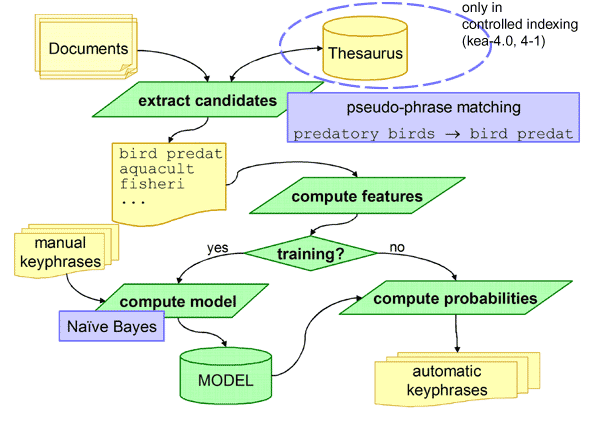
\includegraphics[scale=1]{res/kea_diagram.png}
\caption{Schema di Kea}
\label{fig:kea}
\end{figure}

\section{Metadati di accessibilità per risorse educative}
I progressi nelle tecnologie dell'informazione e della comunicazione, e in particolare nell'ingegneria multimediale, di rete e del software, hanno promosso una nuova generazione di ambienti di apprendimento online.
Molte organizzazioni, sia pubbliche che private, sfruttano le nuove tecnologie per offrire prodotti e servizi educativi e formativi a tutti i livelli. In particolare, l'ampia disponibilità di risorse educative è un obiettivo comune per università, biblioteche, archivi e altre istituzioni ad alta intensità di conoscenza. C'è anche una crescente capacità dei docenti di collaborare con i loro studenti e altri docenti al fine di produrre, condividere e riutilizzare le risorse educative.

In questo contesto, i metadati educativi sono stati riconosciuti come uno dei campi più fruttuosi nella standardizzazione delle tecnologie educative. Tuttavia, l'emergere di grandi raccolte di risorse di apprendimento create attraverso la raccolta e l'aggregazione di metadati ha sollevato importanti preoccupazioni sull'idoneità delle descrizioni delle risorse educative fornite negli schemi di metadati.

Pertanto, la capacità di gestire efficacemente le risorse educative in termini di reperibilità, riutilizzabilità, interoperabilità e accessibilità risiede nell'adozione di uno schema di metadati appropriato, in grado di descriverle adeguatamente. Nonostante ciò, in quest'area è stata fatta solo una piccola ricerca e non esiste una soluzione completa per la gestione dei metadati di accessibilità. L'accessibilità è una caratteristica chiave per promuovere l'istruzione e la formazione inclusive in ambienti di apprendimento virtuali e distribuiti in cui esiste una grande diversità nelle esigenze e nelle preferenze di accessibilità degli studenti.

Storicamente, la tecnologia e la sua funzionalità nel processo di insegnamento e apprendimento hanno offerto agli studenti una varietà di possibilità riguardo alle esperienze di interazione in base alle loro esigenze e preferenze di apprendimento. Il primo tentativo all'utilizzo delle risorse educative nell'ambito della formazione a distanza risale al 1728. Si trattava di corrispondenza stampata. Nel 1971, la British Broadcasting Corporation (BBC) iniziò a trasmettere in televisione i materiali didattici della Open University sotto forma di conferenze registrate. Negli anni '90, diverse università hanno sviluppato tecnologie per gestire le risorse educative digitali dando vita ai Learning Content Management Systems (LCMS) e successivamente ai Learning Management Systems (LMS).

Nel 2002, il Massachusetts Institute of Technology (MIT) ha lanciato l'iniziativa OpenCourseWare, ora Open Education Consortium, per fornire accesso online gratuito alle risorse educative dei corsi del MIT. Nello stesso anno, l'Organizzazione delle Nazioni Unite per l'Educazione, la Scienza e la Cultura (UNESCO) ha coniato Open Educational Resources (OER) per fare riferimento a materiali di apprendimento rilasciati con una licenza aperta che consente l'accesso, l'uso, l'adattamento e la ridistribuzione gratuiti.

Nel 2012, sono stati introdotti i Massive Open Online Courses (MOOC) per integrare i normali corsi universitari. I MOOC differiscono dai tradizionali corsi online ospitati nelle piattaforme LMS in quanto possono avere un numero illimitato di partecipanti, non hanno requisiti di iscrizione e possono essere seguiti gratuitamente pagando facoltativamente solo per certificati ufficiali o servizi extra, come il feedback dell'istruttore.

Nel 2018, l'offerta MOOC globale comprendeva 11.400 corsi online offerti da 900 istituzioni, con 101 milioni di studenti. La natura massiccia e aperta del MOOC implica eterogeneità negli studenti. L'accessibilità dei MOOC e delle risorse educative in essi contenute deve essere garantita, poiché la probabilità che studenti con diverse tipologie di disabilità partecipino a un MOOC è molto maggiore rispetto ai tradizionali corsi in presenza, a distanza o online. 

I MOOC possono facilitare notevolmente l'istruzione delle persone con qualche tipo di disabilità. Tuttavia, affinché uno studente con una disabilità specifica sia in grado di utilizzare un MOOC, le risorse educative devono essere disponibili in formati accessibili e devono esserci meccanismi di metadati per identificare quale risorsa educativa accessibile è più adatta alle diverse esigenze e preferenze di accessibilità, così come diversi stili di apprendimento. Nonostante le opportunità che la tecnologia educativa presenta, è ancora utilizzata per supportare obiettivi, metodi e valutazioni di un curriculum tradizionale. Questo esclude gli studenti che sono ai margini, come le persone con disabilità.

Il processo di descrizione delle risorse educative attraverso alcune specifiche di metadati è solo uno dei passaggi per rendere tali risorse comprensibili agli studenti con disabilità. Affinché le risorse educative siano localizzate, devono essere incorporate in un repository o una piattaforma di apprendimento virtuale (ad esempio Moodle). In entrambi i casi, le risorse educative possono essere caricate per essere condividise con la comunità educativa o per creare un corso. In generale, uno degli strumenti più importanti che ha un repository o una piattaforma di apprendimento virtuale è portare la possibilità di ricerca nei propri contenuti educativi. Se la risorsa educativa è stata descritta con metadati di accessibilità e lo studente ha una descrizione delle sue esigenze e preferenze personali, lo strumento può scegliere le risorse educative più adeguate in modo che lo studente possa comprenderne il contenuto.

Una piattaforma di apprendimento virtuale utilizza una tecnologia che si concentra sullo sviluppo, la gestione e la pubblicazione dei contenuti e delle attività che contribuiscono al processo di insegnamento-apprendimento. Le piattaforme di apprendimento virtuale funzionano con la tecnologia web attraverso un modello client-server e attualmente con la tendenza a fornire servizi distribuiti attraverso il "cloud". Se si tratta di una piattaforma di apprendimento virtuale accessibile, deve essere garantito che tutte le funzionalità possano essere utilizzate da qualsiasi utente, compresi gli utenti con diversità funzionale\cite{edures}.

\subsection{WCAG}
La consapevolezza della diffusa inaccessibilità dei contenuti web ha portato  allo sviluppo di linee guida per gli autori e altri per assicurarsi che i contenuti fossero più accessibili alle persone con disabilità. 

Il World Wide Web Consortium (\textbf{W3C}) ha risposto fondando il programma Web Accessibility Initiative (\textbf{WAI}) al fine di migliorare l'accessibilità dei contenuti web. Il W3C WAI ha sviluppato ampie linee guida su come rendere i contenuti accessibili a tutti i dispositivi, in modo che coloro che utilizzano dispositivi e browser non-standard possano accedervi ugualmente.

Le linee guida per l'accessibilità dei contenuti Web (Web Content Accessibility Guidelines, \textbf{WCAG}), attualmente alla versione 2.1, sono sviluppate attraverso il processo W3C in collaborazione con individui e organizzazioni in tutto il mondo, con l'obiettivo di fornire un unico standard condiviso per l'accessibilità dei contenuti Web che soddisfi le esigenze di individui, organizzazioni e governi a livello internazionale\cite{wcag}.

Al fine di soddisfare le diverse esigenze di questo pubblico, vengono forniti diversi livelli di orientamento:
\begin{itemize}
\item \textbf{Principi}: vi sono innanzitutto quattro principi che forniscono le basi per l'accessibilità del Web:
\begin{itemize}
\item \textit{percepibile}: l'informazione del contenuto non è invisibile a tutti i sensi dell'utente
\item \textit{operabile}: l'interfaccia non deve richiedere un'interazione che un utente non può effettuare
\item \textit{comprensibile}: il contenuto non può essere al di là della comprensione del fruitore
\item \textit{robusto}: il contenuto resta accessibile all'avanzare della tecnologia
\end{itemize}
\item \textbf{Linee guida}: tredici linee guida forniscono gli obiettivi di base verso i quali gli autori dovrebbero lavorare per rendere i contenuti più accessibili agli utenti con disabilità diverse. Le linee guida non sono testabili, ma forniscono il quadro e gli obiettivi generali per aiutare gli autori a comprendere i criteri di successo e a implementare meglio le tecniche.
\item \textbf{Criteri di successo}: per ciascuna linea guida, vengono forniti criteri di successo verificabili per consentire l'utilizzo delle WCAG 2.0 laddove sono necessari requisiti e test di conformità, ad esempio nelle specifiche di progettazione, negli acquisti, nei regolamenti e negli accordi contrattuali. Per soddisfare le esigenze dei diversi gruppi e delle diverse situazioni, vengono definiti tre livelli di conformità: A (minimo), AA e AAA (massimo).
\item \textbf{Tecniche sufficienti e consultive}: per ciascuna delle linee guida e dei criteri di successo nel documento WCAG 2.0 stesso, il gruppo di lavoro ha anche documentato un'ampia varietà di tecniche. Le tecniche sono informative e si dividono in due categorie: quelle sufficienti per soddisfare i \textit{criteri di successo} e quelle \textit{consultive}. Le tecniche consultive vanno oltre quanto richiesto dai singoli criteri di successo e consentono agli autori di affrontare meglio le linee guida. Alcune tecniche consultive affrontano gli ostacoli all'accessibilità che non sono coperti dai criteri di successo verificabili. Laddove sono noti errori comuni, anche questi vengono documentati.
\end{itemize}

\subsection{LOM}
Lo standard \textbf{IEEE LOM} o \textbf{LOM} (Learning Object Metadata) è uno standard aperto che
specifica la sintassi e la semantica degli attributi richiesti per i metadati dei learning object. Lo standard LOM include regole per controllare l'identificazione degli elementi dei dati e dei loro attributi. Fornisce inoltre principi, regole e strutture per la specificazione di quelle stesse risorse. Il suo obiettivo è facilitare la ricerca, la valutazione, il recupero e l'uso dei learning object. Inoltre, IEEE LOM è considerato lo standard più accettato e implementato in più repository di learning objects. Esistono numerose versioni ed estensioni di LOM che sono state sviluppate da IEEE LOM. È organizzato in 9 categorie, ognuna delle quali contiene sottocategorie che possono condividere caratteristiche di base.

\subsection{LRMI}
Questa iniziativa è iniziata nel 2011, il suo scopo era quello di sviluppare una specifica come estensione educativa per Schema.org. Le proprietà LRMI hanno lo scopo di descrivere le risorse educative aggiungendo proprietà specifiche in modo che possano essere facilmente individuate attraverso motori di ricerca e servizi. Le specifiche si basano sul vocabolario fornito da Schema.org e da altri standard. Pertanto, ci sono termini LRMI non inclusi in Schema.org. Con il supporto di Association of Educational Publishers (AEP), Association of American Publishers, Creative Commons (CC), division 501, Bill \& Melinda Gates e William and Flora Hewlett Foundation, LRMI ha sviluppato un framework di metadati per taggare le risorse di apprendimento web. Lo schema LRMI 1.1 è stato adottato da Schema.org nel 2013, che consente alle risorse, attraverso i loro metadati LRMI, di essere riconosciute dai principali motori di ricerca.

\subsection{IMS AfA}
L'obiettivo principale di IMS Access for All (\textbf{AfA}) v3.0 era quello di semplificare lo standard ISO/IEC 24751 a causa delle difficoltà sorte nella pratica. Entrambi, lo standard ISO/IEC 24751 e AfA v3.0, coprono l'intero processo dalla lettura delle esigenze dell'utente al meccanismo di ricerca necessario per trovare i learning object che soddisfano tali esigenze o preferenze. Ha due modelli di dati:
\begin{itemize}
\item Personal Needs and Preferences (PNP): un modello per la descrizione dei bisogni e delle preferenze degli utenti per accedere e interagire con le risorse digitali.
\item Digital Resource Description (DRD): un modello per la descrizione dei metadati di accessibilità per le risorse didattiche digitali.
\end{itemize}

La specifica AfA DRD definisce i metadati di accessibilità per una risorsa che verrà utilizzata per la ricerca e l'uso della risorsa di apprendimento più adatta per ciascun utente secondo i PNP. Lo strumento LOMPAD è stato abilitato per introdurre metadati di accessibilità (oltre ai metadati ordinari) secondo la specifica IMS 3.0.

Il modo di lavorare con oggetti di apprendimento accessibili richiede la creazione di oggetti di apprendimento originali e adattati. Esistono diversi strumenti che ne facilitano la creazione. Una risorsa originale corrisponde a una risorsa iniziale, mentre una risorsa adattata presenta le stesse informazioni educative della risorsa iniziale o originale ma con caratteristiche diverse, come la modalità sensoriale di accesso alla risorsa, la lingua, ecc. Ad esempio, un file in formato pdf come risorsa originale e una descrizione audio del suo contenuto come risorsa adattata. Il primo presenta l'accesso testuale mentre l'adattamento presenta l'accesso uditivo allo stesso contenuto educativo. Pertanto, le risorse originali possono avere un numero qualsiasi di adattamenti, totali o parziali.

I metadati possono supportare le informazioni adeguate delle risorse originali, come la modalità di accesso (vista, udito, alfabetizzazione, presentazione, fattibilità della trasformazione, controllo, flessibilità, adattamenti, strumenti di aiuto, ecc.) e informazioni rilevanti sulle risorse adattate, come il tipo di adattamento (sottotitoli, lingua dei segni), l'estensione, e la descrizione. Una fusione di risorse, metadati descrittivi e metadati di accessibilità corrisponde al consolidamento di una fonte di archivi accessibili che rafforzi la ricerca di learning object secondo i bisogni educativi speciali.

\begin{figure}[H]
\centering
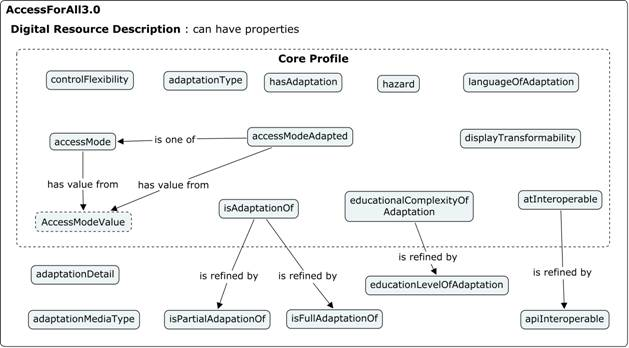
\includegraphics[scale=0.7]{res/drd.png}
\caption{Proprietà del modello DRD}
\label{fig:drd}
\end{figure}

Lo scopo della specifica AfA PNP è quello di consentire la definizione dei bisogni personali degli studenti (o quelli relativi agli ambienti della disabilità). I PNP vengono utilizzati in combinazione con la specifica AfA DRD per fornire risorse digitali che soddisfino le esigenze di un utente e/o le sue preferenze. I PNP dello studente o dell'utente definiscono le sue preferenze nell'utilizzo delle diverse modalità sensoriali per la percezione delle informazioni. Il metodo suggerito per generare i PNP dello studente è la presentazione di un modulo con diverse opzioni sulla modalità sensoriale preferita per l'accesso alle informazioni. I PNP saranno generati dalle risposte dello studente alle domande nel modulo.

I principi di accessibilità sull'e-learning sono focalizzati sulla fornitura di opzioni di personalizzazione basate sulle preferenze dell'utente, sugli equivalenti dei contenuti e sulla compatibilità con l'aiuto tecnico e l'accesso completo alla tastiera, oltre a fornire informazioni sul contesto e offrire supporto in modo che l'utente possa seguire specifiche su direttive e/o norme di organi di governo come IMS.

\begin{figure}[H]
\centering
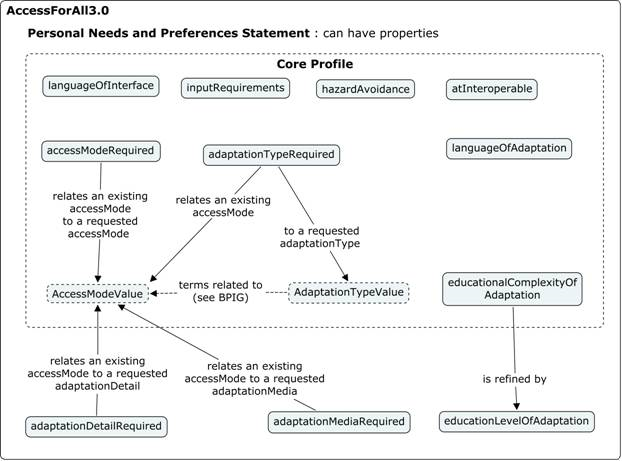
\includegraphics[scale=0.7]{res/pnp.png}
\caption{Proprietà del modello PNP}
\label{fig:pnp}
\end{figure}

\subsection{Schema.org}
\textbf{Schema.org} è una comunità responsabile della creazione, della manutenzione e della promozione di schemi di metadati per dati strutturati pubblicati su Internet. L'aspetto più interessante di Schema.org è che riceve il supporto di grandi aziende come Google, Microsoft e Yahoo. Ciò significa che l'incorporazione di metadati nei contenuti pubblicati su Internet è essenziale per poterli categorizzare e descrivere le loro caratteristiche di accessibilità.

I formati più utilizzati per fare annotazioni semantiche sono microdati, microformati, JSON-LD e RDFa.
Il formato dei microdati è stato sviluppato nell'ambito della standardizzazione di HTML5 per la marcatura dei contenuti web. I microdati sono costituiti da un gruppo di coppie nome-valore; i gruppi sono chiamati elementi e ogni coppia nome-valore è una proprietà. Gli elementi sono definiti dai seguenti cinque attributi: \textit{itemscope}, \textit{itemtype}, \textit{itemid}, \textit{itemprop} e \textit{itemref}. Queste annotazioni forniscono la semantica attraverso la terminologia e le proprietà di un dominio di rappresentazione della conoscenza, comprese le sue relazioni.

La specifica Schema.org stabilisce una raccolta di vocabolari condivisi che includono proprietà per descrivere alcune caratteristiche di diversi tipi di contenuto web. Queste descrizioni possono essere comprese dai principali motori di ricerca. Nel caso di Google, il suo motore di ricerca utilizza i microdati HTML5 di Schema.org per migliorare i risultati delle sue ricerche e consente a chiunque di effettuare una ricerca personalizzata utilizzando i diversi schemi di Schema.org per limitare le ricerche.

Per definire i metadati di accessibilità in Schema.org, sono definiti diversi tipi di contenuto web e possono essere
classificati utilizzando schemi di metadati.
I tipi possono avere sottotipi, ad esempio "CreativeWork" ha il tipo "MediaObject" e questo ha a sua volta "VideoObject".
I metadati di accessibilità definiti da Schema.org si basano su quelli specificati per IMS AfA v3.0 DRD, ma ne è stato selezionato un sottoinsieme significativo. Ciascuno di questi metadati può avere un possibile valore definito nella specifica. In questo modo si possono determinare le caratteristiche di accessibilità di qualsiasi risorsa digitale pubblicata sul web.

\begin{figure}[H]
\centering
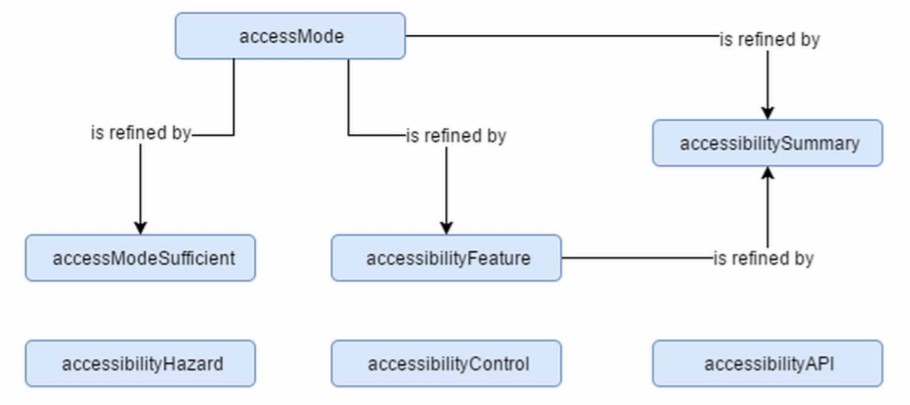
\includegraphics[scale=0.7]{res/schemaorg.png}
\caption{Metadati di accessibilità di CreativeWork da Schema.org}
\label{fig:schemaorg}
\end{figure}